\subsection{Explicación del algoritmo realizado}
Para resolver el algoritmo presentado anteriormente con una técnica golosa, decidimos utilizar el procedimiento que se presenta a continuación:\newline
\newline
\begin{algorithm}[H]
    \SetAlgoLined
    \caption{HeurísticaGolosa}
    \KwIn{\textbf{Grafo} $g$}
    \KwOut{\textbf{Conj(nodos)} $clique$}
	Entero $nodoDeMayorGrado$ = nodoDeMasGrado($g$)\\
	Grafo $cliqueHastaAhora$ = $\emptyset$\\
	agregar($v$, $cliqueHastaAhora$)\\
	\ForAll{$u \in$ adyacentes(nodoDeMayorGrado, nodos($g$))}{
		\If{forma una clique($g$, agregar($u$, $cliqueHastaAhora$)) $\land$ frontera($g$, agregar($u$, $cliqueHastaAhora$) $>$ frontera($cliqueHastaAhora$)}{
		agregar($u$, $cliqueHastaAhora$)}}
\textbf{devolver} $cliqueHastaAhora$
\end{algorithm}

donde $nodoDeMasGrado$ consiste en una función que toma el nodo del grafo cuyo grado es el mayor, $frontera$ es una función que calcula la frontera de un conjunto de nodos dentro de un grafo y $adyacentes$ consiste en una lista de nodos adyacentes a un determinado nodo.\newline


\subsection{Complejidad Temporal}
Veamos cuál es la complejidad temporal del algoritmo realizado:
\begin{itemize}
\item En primer lugar, el algoritmo utiliza la función $esClique$ para verificar si un conjunto de nodos de un grafo forman una clique. Dicha función consiste en dos ciclos, uno dentro de otro, que iteran cantidad de la clique veces, lo que resulta $\mathcal{O}(n^2)$ como peor caso. Dentro de los ciclos mencionados, se realizan dos comparaciones, donde una de ellas utiliza la función $sonVecinos$ ($\mathcal{O}(1)$). Luego, la complejidad temporal de la función $esClique$ resulta $\mathcal{O}(n^2)*\mathcal{O}(1)$ = $\mathcal{O}(n^2)$.

\item Por otro lado, la función $greedySearch$ crea un vector inicializado en 1 de tamaño $nodoDeMayorGrado$ ($\mathcal{O}(n)$) y un entero al que se le asigna el valor de la frontera de $cliqueHastaAhora$. Dicho valor se calcula con $frontera$ en $\mathcal{O}(n)$. Luego, se ejecuta un ciclo con la cantidad de nodos ($\mathcal{O}(n)$) en el que se realiza un $push\_back$ ($\mathcal{O}(1)$ amortizado\footnote{http://www.cplusplus.com/reference/vector/vector/push\_back/}) y se verifica que el vector $cliqueHastaAhora$ sea una clique con la función $esClique$ ($\mathcal{O}(n^2)$). Si dicha verificación resulta afirmativa, se compara la frontera de $cliqueHastaAhora$ con un entero ($\mathcal{O}(n)$) y luego se le asigna la nueva frontera a $fronteraHastaAhora$ (con la función $frontera$ en $\mathcal{O}(n)$). Caso contrario, se retira el último elemento agregado a la clique con $pop\_back()$ ($\mathcal{O}(1)$\footnote{http://www.cplusplus.com/reference/vector/vector/pop\_back/}).\newline
\newline
Luego, la complejidad temporal de la función $greedySearch$ resulta $2^*\mathcal{O}(n)+\mathcal{O}(n)^*\mathcal{O}(n)^*\mathcal{O}(n^2)$ = $\mathcal{O}(n^4)$.

\end{itemize}
\subsection{Instancias problemáticas}
La Heurística Golosa realizada falla muy fácilmente. Por ejemplo, cuando la clique de máxima frontera no contiene al nodo de mayor grado, ésta devuelve un resultado erróneo. Dado que esta característica afecta a una gran cantidad de grafos, dicho problema implica una cantidad asintótica de fallas por parte de la Heurística Golosa realizada. 
\subsection{Experimentación}
Para la experimentación de la Heurística Golosa, nos limitamos a realizar un gráfico comparativo para grafos aleatorios entre la cantidad de nodos agregados respecto del tiempo de ejecución. Para ello, utilizamos un generador de grafos y aumentamos de forma paulatina la cantidad de nodos, respetando una densidad del 50\% para las aristas.\newline
Las mediciones de tiempo en nanosegundos se realizaron con la función $high\ resolution\ clock$\footnote{http://en.cppreference.com/w/cpp/chrono/high\_resolution\_clock} de la librería $Chrono$ de $C++$. 

Las funciones de complejidad con las que se compararon nuestros gráficos de tiempo fueron ajustadas por algoritmos matemáticos (proporcionados por \textbf{sci davis}). Dichos algoritmos se encargaron de multiplicarle y sumarle constantes a las funciones con el fin de que éstas se ajustaran a nuestros resultados sin modificar el comportamiento de las funciones utilizadas para comparar.

\begin{figure}[H] %[h] Aqui [b] para button [t] para top
\begin{center}
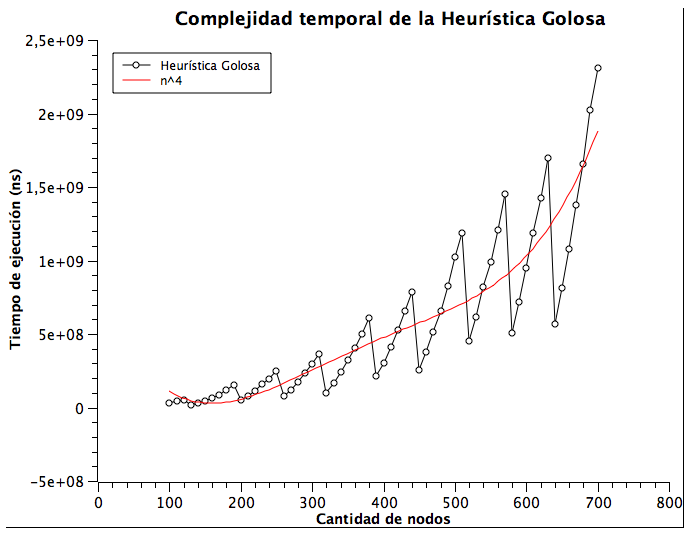
\includegraphics[width=350pt]{../imgs/complejidad_goloso.png}
\caption{Complejidad Temporal de la Heurística Golosa.}
\end{center}
\end{figure}

